\section{Concorrenza}

La concorrenza è un concetto fondamentale nell'ambito
dello sviluppo software, si riferisce alla capacità
di eseguire più attività contemporaneamente.
Questo è particolarmente importante in applicazione
che devono gestire molteplici operazioni in parallelo
come ad esempio un server web, applicazioni di
elaborazione dati.

La concorrenza consente a un programma di sfruttare appieno
le risorse disponibili, aumentando l'efficienza e migliorando
le prestazioni complessive.
Inoltre, permette di creare sistemi più reattivi e
scalabili, in grado di gestire un numero crescente di
richieste senza compromettere le prestazioni.

In generale, la gestione della concorrenza può essere complessa
e soggetta a errori o comportamenti indeterminati, infatti,
più processi o thread possono interagire tra loro in modo
imprevedibile, essendo così costretti a usare tecniche di
locking in concomitanza di memoria condivisa trà più thread.

Nel contesto di Elixir, la concorrenza è un concetto centrale
e viene gestita attraverso il modello di programmazione
basato su processi leggeri, tutti isolati tra loro con il proprio
stack ed il proprio heap.

% ------------------------------------------------------

\subsection{La concorrenza in Beam}

La concorrenza gioca un ruolo chiave per un software
che vuole essere altamente responsivo.
La concorrenza fa uso dei cosiddetti processi leggeri
nella piattaforma Erlang, non sono processi del 
sistema operativo, ma processi della
VM Beam, chiamato processo e non thread in quanto non
condividono memoria e sono completamente
isolati tra di loro.

Un server tipico deve gestire migliaia di richieste, e
gestirle concorrenzialmente è essenziale per non far
rimanere in attesa il client. Quello che si vuole è
gestirli parallelamente il più possibile sfruttando
più risorse della Cpu disponibile.
Quello che fa la macchina virtuale per noi è permetterci
la scalabilità,più richieste allora più risorse da allocare.

Inoltre, siccome il processo è isolato, un errore in una richiesta
può essere localizzato senza avere impatto
sul resto del sistema, così creando anche un sistema robusto
agli errori.

Un processo appena creato occupa in memoria 326 words \cite{ErlangPr21:online},
quindi in una macchina a 64 bit occupa 2608 byte.
Lo si può vedere in Elixir facilmente nell'esempio \ref{lst:memoryoneprocess}

\begin{lstlisting}[language=elixir, caption={Memoria in un processo},captionpos=b,
	label={lst:memoryoneprocess}]
defmodule Examples.Memory do
  def mypid do
    receive do
      :stop -> :exit
      _ -> mypid()
    end
  end
 
  def benchmark do
    pid = spawn(fn -> mypid() end)
    {_,byte_used} = :erlang.process_info(pid,:memory)
    IO.puts("La memoria usata dal processo e': #{byte_used} byte")
    send pid, :stop
  end
end
\end{lstlisting}

Infatti l'output ottenuto dall'esempio \ref{lst:memoryoneprocess}
\begin{lstlisting}[language=none]
iex> Examples.Memory.benchmark
La memoria usata dal processo e': 2640 byte
:stop
\end{lstlisting}
	
Si nota dall'output dell'esempio che la memoria utilizzata
è leggermente superiore della memoria minima dichiarata,
infatti il processo non fa nulla di particolare oltre
ad aspettare il messaggio di ":stop".
È da notare che è proprio questa leggerezza nei processi che
permette al linguaggio di essere orientato alla concorrenza,
e poter usare i processi con più leggerezza rispetto
ad altri meccanismi di altri linguaggi che usano i thread,
Un altro punto da notare è che si può migliorare significativamente
la reattività del programma ma non l'efficienza totale del
sistema, infatti non tutti i processi
sono eseguiti in parallelo, quindi in una macchina con quattro
processori non si possono eseguire più di 4 processi per volta
ed in un normale software Elixir è normale avere migliaia di
processi che lavorano.

Facendo un esempio con una Cpu dual-core,
i processi vengono eseguiti concorrenzialmente e gestiti
dagli Scheduler della VM,
in figura \ref{fig:concorrenza_beam} è mostrato come
la VM gestisce i processi di default.

\begin{figure}[!htp]
    \centering
    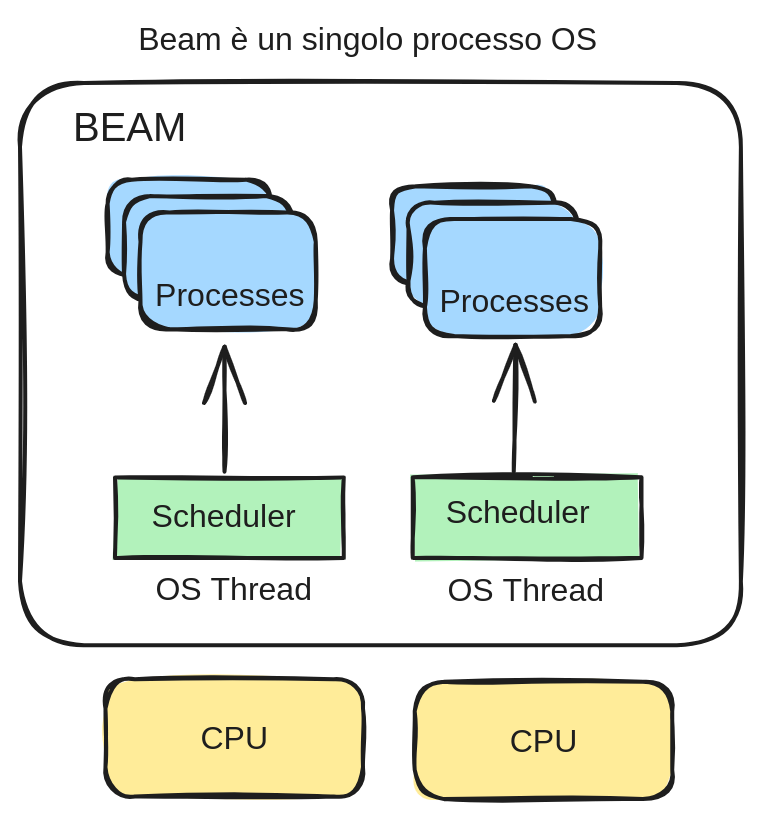
\includegraphics[keepaspectratio=true,scale=0.25]{images/beam_concurrency.png}
	\caption{Concorrenza nella VM Beam \cite{elixirInAction5}}
  	\label{fig:concorrenza_beam}
\end{figure}


%--------------------------------------------------------------

\subsection{Concorrenza basata su attori}

Elixir usa un modello di concorrenza basato su attori,
gli attori sono entità di elaborazione indipendenti
che eseguono operazioni in modo asincrono, questi attori
non sono altro che processi che vengono identificati
attraverso un \textbf{PID} univoco. Come già detto
sono isolati l'uno dall'altro e
comunicano solo attraverso lo scambio di messaggi,
questo scambio avviene attraverso
dei canali di comunicazione detti \textbf{"mailbox"}.
Ogni processo ha una propria mailbox dove avviene la
ricezione del messaggio da parte di altri processi.

Conoscendo il PID di un processo può avvenire la comunicazione
attraverso la primitiva fornita dal linguaggio \textbf{send/2}
che permette di inviare un messaggio ad un processo
come avviene nell'esempio \ref{lst:memoryoneprocess}, dove
il processo principale crea un processo che rimane in ascolto
tramite il blocco \textbf{receive/1},
fin quando non riceve il messaggio di \textbf{:stop} e il processo
viente terminato.

Se non ci sono messaggi nella mailbox, il processo aspetta fino a
quando non arriva un messaggio, in particolare, 
nell'esempio tutti i messaggi che
non siano :stop, verranno ignorati continuando ad ascoltare altri
messaggi.

\subsubsection{Process Linking}

I processi sono isolati, ma si può legare un processo
al processo chiamante tramite un operazione di Process linking,
questo per sapere se il processo va in errore
oppure termina per un comportamento imprevisto,
legando i processi si può propagare l'errore nel caso
uno dei due processi non ha senso di esistere preso da solo.

Spesso i processi vengono legati ad un Supervisor, che
lascerà andare in errore i processi figli, e si occuperà
semplicemente di riavviarli seguendo una strategia scelta.
Questa è la filosofia "Let it Crash"
di Erlang, che si contrappone alla gestione delle eccezioni
di altri linguaggi. Si veda l'esempio \ref{lst:processlinking}

\begin{lstlisting}[language=elixir, caption={Process linking},captionpos=b,
	label={lst:processlinking}]
iex>spawn(fn -> raise "oops" end)
#PID<0.58.0>
	
[error] Process #PID<0.58.00> raised an exception
** (RuntimeError) oops
	(stdlib) erl_eval.erl:668: :erl_eval.do_apply/6

iex(2)spawn_link(fn -> raise "ooops" end)

17:37:50.425 [error] Process #PID<0.113.0> raised an exception
** (RuntimeError) ooops
** (EXIT from #PID<0.110.0>) shell process 
** exited with reason: {%RuntimeError{message: "ooops"}, []}

iex(2)
\end{lstlisting}

Notiamo nell'esempio \ref{lst:processlinking} che con il comando
la funzione spawn\_link/1 il processo va in errore e propaga
l'errore all'ambiente interattivo iex, riavviando anche
l'ambiente iex.

Si nota in conclusione al paragrafo che è possibile
gestire migliaia di processi molto facilmente senza
incrementare in modo considerevole le risorse in memoria grazie
ai processi leggeri, permettendo
di sviluppare un software orientanto alla concorrenza,
tutto è facilitato dall'isolamento di ogni processo che 
permette di non preoccuparsi di meccanismi di locking e sincronizzazine.
Elixir permette di non preoccuparci di come scalare
le risorse hardware, potendo dare responsabilità ad altri
processi creando più flussi di esecuzione.